\section{Experiments}
\label{sec:experiments}

The evaluation tests whether PCU-Select preserves per-PEFT LESS's average downstream quality, reduces the marginal cost of adding a PEFT, and transfers to new configurations according to their structural support in the training registry. After establishing quality and cost, we examine whether conditioning produces target-specific subsets and identify which components sustain the reusable scorer.

\subsection{Setup}

We evaluate Llama-2-7B~\cite{touvron2023llama2} on GSM8K, HumanEval, MMLU, and TyDiQA~\cite{cobbe2021gsm8k,chen2021humaneval,hendrycks2021mmlu,clark2020tydiqa}, using exact match, Pass@1, accuracy, and F1, respectively. We express these scores as percentages and use their equal-weight macro-average only as a registry-level summary. Per-task results appear in Supplementary Table~S1. From a decontaminated pool of 300K mixed instruction examples, every selector chooses 10\%; the supplementary material gives the reproducibility protocol.

The main comparison covers five configurations seen during scorer training: attention and MLP LoRA, (IA)$^3$, and adapters. The transfer study holds out configurations that vary rank, placement, learning rate, or family. Its unseen-family slice includes Prefix Tuning, P-Tuning, and LN Tuning~\cite{wang2022lntuning}. We instantiate LN Tuning on Llama-2 by updating the scale parameters of both RMSNorm modules in every Transformer block and excluding the final model-level RMSNorm~\cite{touvron2023llama2}. Supplementary Table~S3 lists the full 17-configuration registry.

The four baselines differ in target specificity. \textbf{Random} uses neither task nor PEFT information. \textbf{RDS+}, our representation-similarity baseline, ranks frozen semantic embeddings by similarity to the task-sketch mean but ignores the PEFT configuration. \textbf{Influence}, our shared-datastore gradient baseline, ranks projected base-model gradients from one PEFT-agnostic datastore. \textbf{LESS}, our per-PEFT implementation of gradient-influence selection~\cite{xia2024less}, warms up each target adapter, builds an Adam-preconditioned gradient datastore, and ranks examples by sketch influence. PCU-Select uses its conditional scorer, uncertainty penalty, and adaptive semantic-cluster quotas. The supplementary material gives full specifications.

We hold the backbone, PEFT recipe, training steps, and evaluation protocol constant, so only the selected subset changes. The main table varies target-training seeds 0, 1, and 2 while fixing the selector, scorer, sketch, and pool at seed 0. Matched seeds give every selector the same training randomness. We obtain each descriptive 95\% interval by resampling the evaluated PEFT--task cells under this fixed selection pipeline.

\subsection{PCU-Select Near-Ties Per-PEFT LESS}
\label{sec:quality}

\begin{table*}[t]
\centering
\small
\setlength{\tabcolsep}{4pt}
\begin{tabular}{lrrrrrr}
\toprule
Method & AD-b64 & IA3-attnmlp & L-r16-qkvo & L-r8-mlp & L-r8-qv & Avg. \\
\midrule
Random & 32.79$\pm$0.38 & 31.74$\pm$0.13 & 33.11$\pm$0.23 & 31.97$\pm$0.21 & 31.82$\pm$0.16 & 32.29$\pm$0.16 \\
RDS+ & 35.27$\pm$0.23 & 33.54$\pm$0.26 & 35.00$\pm$0.29 & 34.46$\pm$0.21 & 33.91$\pm$0.17 & 34.44$\pm$0.13 \\
Influence & 35.08$\pm$0.27 & 33.84$\pm$0.26 & 35.24$\pm$0.19 & 34.69$\pm$0.13 & 34.53$\pm$0.22 & 34.68$\pm$0.11 \\
LESS & 35.52$\pm$0.20 & 34.44$\pm$0.13 & 35.80$\pm$0.15 & \textbf{35.13$\pm$0.14} & 34.80$\pm$0.37 & 35.14$\pm$0.14 \\
PCU-Select & \textbf{35.61$\pm$0.40} & \textbf{34.60$\pm$0.21} & \textbf{35.93$\pm$0.30} & 34.56$\pm$0.23 & \textbf{35.18$\pm$0.31} & \textbf{35.18$\pm$0.16} \\
\bottomrule
\end{tabular}
\caption{Each PEFT column reports the equal-weight macro-average of the four task-native percentage scores. Values are mean $\pm$ standard deviation across three matched downstream-training seeds; the selector, task sketch, candidate pool, and scorer are fixed. Across the 20 configuration--task cells, the paired PCU-Select-minus-LESS difference is $+0.04$ points, with a descriptive 95\% interval of $[-0.26,+0.33]$.}
\label{tab:main-results}
\end{table*}


Table~\ref{tab:main-results} shows that PCU-Select improves on the PEFT-agnostic baselines and remains close to target-specific LESS. It gains 0.74 points over RDS+ and wins 17 of 20 PEFT$\times$task cells, with descriptive interval $[+0.38,+1.06]$. It gains 0.50 points over Influence and wins 18 cells, with interval $[+0.21,+0.75]$. Its mean is 0.04 points above LESS, with interval $[-0.26,+0.33]$ and 10 wins in 20 cells.

The LESS comparison varies across tasks. PCU-Select leads on MMLU, has task-level descriptive intervals that cross zero on GSM8K and HumanEval, and trails on TyDiQA and MLP-only LoRA. Task-grouped resampling yields $[-0.15,+0.22]$ for the aggregate gap (Supplementary Table~S1). Together, these results show that PCU-Select improves both PEFT-agnostic baselines and near-ties per-PEFT LESS.

\subsection{Amortization Cuts Four-Task PEFT Onboarding Cost by 42$\times$}
\label{sec:reuse}

\begin{table}[t]
\centering
\small
\setlength{\tabcolsep}{2pt}
\begin{tabular}{lrrrrr}
\toprule
Method & Fixed & Marg. & Total & Quality & Gap \\
\midrule
Random          &  0.0 &  0.0 &   0.0 & 32.29 & $-2.85$ \\
RDS+            &  1.6 &  0.0 &   1.6 & 34.44 & $-0.70$ \\
Influence       & 48.8 &  0.0 &  48.8 & 34.68 & $-0.46$ \\
Reuse-one-LESS  & 63.2 &  0.0 &  63.2 & 34.24 & $-0.90$ \\
\midrule
LESS            &  0.0 & 63.2 & 316.0 & 35.14 & $\phantom{+}0.00$ \\
PCU-Select      & 144.0 & \textbf{1.51} &  151.6 & \textbf{35.18} & $+0.04$ \\
\bottomrule
\end{tabular}
\caption{Quality and selection cost across five seen PEFTs. Costs are GPU-hours
and exclude downstream tuning; \emph{Gap} is the paired difference from
LESS in task-native points. Boldface marks the best quality and marginal cost.}
\label{tab:quality-cost-headline}
\end{table}


Table~\ref{tab:quality-cost-headline} separates \emph{fixed/shared} cost, paid once, from \emph{marginal} cost, paid for each new PEFT. All selector costs exclude the shared 12.8 GPU-hour downstream run. PCU-Select and per-PEFT LESS have near-tied average quality but distribute selection cost differently. LESS has no fixed cost and spends 63.2 GPU-hours per four-task configuration. PCU-Select pays 144.0 GPU-hours once, then 1.51 GPU-hours per new configuration: a $42\times$ lower marginal cost.

The gap comes from configuration reuse. Adding a task to an existing PEFT costs one online-selection pass: 0.38 GPU-hours for PCU-Select and 0.30 for LESS. The PCU-Select value rounds the exact average per-task cost of 0.3775. Adding a PEFT forces LESS to rebuild its datastore, whereas PCU-Select reuses the scorer (Supplementary Table~S5). The cost benefit therefore comes from cross-PEFT reuse.

The fixed-subset shortcut trades away quality. \textbf{Reuse-one-LESS} applies one LESS subset to all five targets; it costs 63.2 GPU-hours but averages 34.24, below RDS+ at 34.44. Reusing a subset selected for one trainable subspace removes the target condition. PCU-Select produces a distinct subset for each target and retains LESS-level average quality.

The measured costs break even at 2.33 four-task configurations; the supplementary material gives the derivation. Serving the five-PEFT registry costs 151.6 GPU-hours with PCU-Select and 316.0 with LESS, a $2.09\times$ reduction.
For targets far from the training registry, optional calibration uses 500 \emph{reduced calibration labels} from one warm anchor and one update step. This procedure costs 1.05 GPU-hours per $(p,t)$, one quarter of the $\approx4.2$ GPU-hours for the full routine. It shifts the worst-case break-even point to 2.50 configurations. For supported four-task configurations that require no calibration, PCU-Select's marginal selection cost is $42\times$ lower than per-PEFT LESS.

\subsection{PEFT Conditioning Produces Target-Specific Subsets}
\label{sec:conditioning}

Selecting for the target LoRA configuration beats reusing another configuration's subset by 1.45 points (21.25 versus 19.79; Supplementary Figure~S1).
Subset differences increase with structural configuration distance, supporting PEFT-conditioned utility; Supplementary Figure~S1 reports the Jaccard and leave-one-configuration-out analyses.

\subsection{Reduced Calibration Narrows the L1 and LN-Tuning Gaps}
\label{sec:transfer}

We next test whether the structural code guides transfer beyond seen targets. Before evaluation, we fix three support levels: L0 resembles a seen configuration, L1 makes a larger shift within a seen family, and L2 introduces an unseen family. Supplementary Table~S3 lists the registry.

\begin{figure}[t]
\centering
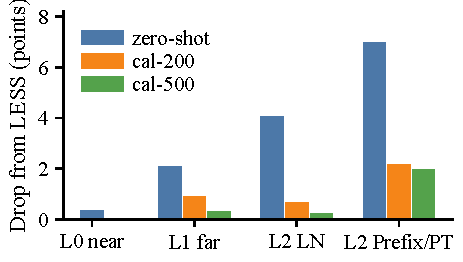
\includegraphics[width=.70\columnwidth]{Figures/fig_ood_calibration.pdf}
\caption{Bars show the three-seed mean of reference minus PCU-Select on GSM8K, HumanEval, and MMLU; Supplementary Table~S11 reports SD. Lower is better; the horizontal axis marks parity. LESS is the reference except for Prefix/P-Tuning (RDS+); L0 is zero-shot only.}
\label{fig:ood-calibration}
\end{figure}

Against LESS, the zero-shot drop grows with structural distance from L0 through L1 to LN Tuning (Figure~\ref{fig:ood-calibration}; Supplementary Table~S11). L0 trails LESS by 0.34 points zero-shot. Adding 500 reduced calibration labels decreases the L1 drop from 2.08 to 0.30 points and the LN-Tuning drop from 4.08 to 0.23. We compare Prefix/P-Tuning with RDS+ because compatible calibration labels are unavailable; their zero-shot score is 6.97 points lower.

The 500-label reduced-calibration setting costs 1.05 GPU-hours per PEFT--task pair, one quarter of the offline routine. Zero-shot covers near-support targets; reduced calibration nearly closes the tested L1 and LN-Tuning mean drops when labels are compatible.

\subsection{Ablations Identify the Useful Components}
\label{sec:ablation}

Removing the PEFT code causes the largest downstream drop, 1.37 points; the task sketch, both label sources, and adaptive semantic coverage also improve quality.
Supplementary Table~S9 reports the full ablation on GSM8K and HumanEval with two representative PEFTs.

\subsection{Limitations}

Our evaluation covers one backbone family, four tasks, and a finite registry; short-update labels approximate contribution after full training. The current method falls back to a per-target selector for Prefix/P-Tuning because compatible calibration labels are unavailable. Its cost advantage begins after 2.33 four-task configurations for direct scoring and 2.50 under the reported worst-case calibration cost, and it applies when the registry requires LESS-level selection quality.
